\documentclass[twocolumn]{article}
\usepackage{caption}
\usepackage[utf8]{inputenc}
\usepackage{amsmath}
\usepackage[margin=1in]{geometry}
\usepackage{changepage}
\usepackage{titling}
\usepackage{ragged2e}
\usepackage{abstract}
\usepackage{enumitem}
%\usepackage{wrapfig}
\usepackage{graphicx}
\usepackage{hyperref}
\renewcommand{\thesection}{\Roman{section}}
\setlength{\columnsep}{1cm}
\setlength\parindent{5pt}
\DeclareMathOperator{\arccosh}{arccosh}
\begin{document}
\twocolumn[
\begin{@twocolumnfalse}
\title{\Large{\textbf{AC and DC Hall Effect experiment on a 300$\mu m$ 
Si doped wafer}}}
\author{Herbert D. Ludowieg}
\setlength{\droptitle}{-0.65in}
\maketitle
\begin{onecolabstract}
%\begin{adjustwidth}{0.5in}{0.5in}
\justify
The Hall Effect is a phenomena of solid materials that has been in use since 
the turn of the century. In this experiment we used the AC and DC hall effect 
to see the properties of a Si doped semiconductor sample including: the type 
of semiconductor, carrier mobility and density and the resistivity of the 
sample. It was determined the sample was an n-type emiconductor, with a 
temperature dependent carrier density with values: 3.08$x10^{20}$ 
$\pm$ 0.09$x10^{20}$ at 80K, 3.1$x10^{20}$ $\pm$ 0.3$x10^{20}$ at 100K, 
3.06$x10^{20}$ $\pm$ 0.07$x10^{20}$ at 120K, 2.83$x10^{20}$ $\pm$ 
0.04$x10^{20}$ at 140K, 2.8$x10^{20}$ $\pm$ 0.1$x10^{20}$ at 160K, 
3.5$x10^{20}$ $\pm$ 0.1$x10^{20}$ at 180K, 3.12$x10^{20}$ $\pm$ 0.07$x10^{20}$ 
at 200K, 3.8$x10^{20}$ $\pm$ 0.2$x10^{20}$ at 220K, 3.8$x10^{20}$ $\pm$ 
0.2$x10^{20}$ at 240K and 3.9$x10^{20}$ $\pm$ 0.2$x10^{20}$ at 260K. With 
temperature dependent values of: 1.44$x10^{-2}$              
$\pm$ 0.05$x10^{-2}$ at 80K, 1.5$x10^{-2}$ $\pm$ 0.1$x10^{-2}$ at 100K, 
1.49$x10^{-2}$ $\pm$ 0.03$x10^{-2}$ at 120K, 1.63$x10^{-2}$ $\pm$ 
0.03$x10^{-2}$ at 140K, 1.7$x10^{-2}$ $\pm$ 0.07$x10^{-2}$ at 160K, 
1.47$x10^{-2}$ $\pm$ 0.06$x10^{-2}$ at 180K, 1.77$x10^{-2}$ $\pm$ 
0.04$x10^{-2}$ at 200K, 1.57$x10^{-2}$ $\pm$ 0.07$x10^{-2}$ at 220K, 
1.68$x10^{-2}$ $\pm$ 0.09$x10^{-2}$ at 240K and 1.69$x10^{-2}$ $\pm$ 
0.07$x10^{-2}$ at 260K.\\ \\
%\end{adjustwidth}
\end{onecolabstract}
\end{@twocolumnfalse}
]
%\begin{multicols}{2}
\justify
\section{Introduction}
The hall Effect was discovered by Edwin H. Hall in 1879, who at the time was 
studying Rowland at Johns Hopkins University. During those days no one knew of 
the electron and by extension how it was that conduction actually happened. 
Due to this it took almost 50 years until the Hall Effect was fully understood 
with the formulation of quantum mechanics. The results that were gotten from 
the experiment were generally not very well understood \cite{ref:1}.
\\
However, when quantum mechanics was formulated and the Hall Effect became fully 
understood it began to be employed in the study of semiconductors. It was here 
that it fullfilled its promise in the study of the concentration and sign of 
charge carriers \cite{ref:1}. Both of which are to be found in this experiment. 
\\
There are four different types of materials: insulators and superconductors, 
semiconductors and conductors. The difference between all of these are the 
resistivity and conductivity values for them. Insulators and superconductors 
behave in a very similar fashion in that they allow almost no current to pass 
through them, they have near infinite resistivities and near zero conductivity 
values. Conductors are the polar opposite of them having very low resistivity 
values and extremely high conductivity. Semiconductors are the middle ground 
where the two meet having finite resistivity and conductivity values.
\\
Semiconductors are an integral 
part in our daily lives since they have been in wide use in electronics such 
as: computers, cell phones and LED bulbs. The Hall Effect has given a far 
reaching insight into how and why it is that the properties listed above 
display such distinct behaviors.
\\
For the experiment a large electromagnet with a magnetic field range of 0 T to 
0.6678 T was used to create a homogenous strong magnetic field. To receive the 
signals a lock-in amplifier was used for the AC Hall Voltage measurements and a 
simple multi-meter was used to measure the DC Hall Voltage measurements. The 
temperature of the sample could also be controlled via a PID temperature 
controller that allowed to heat up the sample and it was cooled down through 
the use of Liquid Nitrogen (LN). The sample was housed in a cryostat chamber 
containing a very dilute Helium gas concentration to be a thermal contact 
between the inner chamber and the LN.
\\
The sample was a Silicon doped semiconductor which we put at cryogenic 
temperatures and in a high intensity magnetic field to perform the measurements.
\section{Theory}
%\begin{wrapfigure}{l}{0pt}
\begin{figure*}
\begin{minipage}[t]{0.46\textwidth}
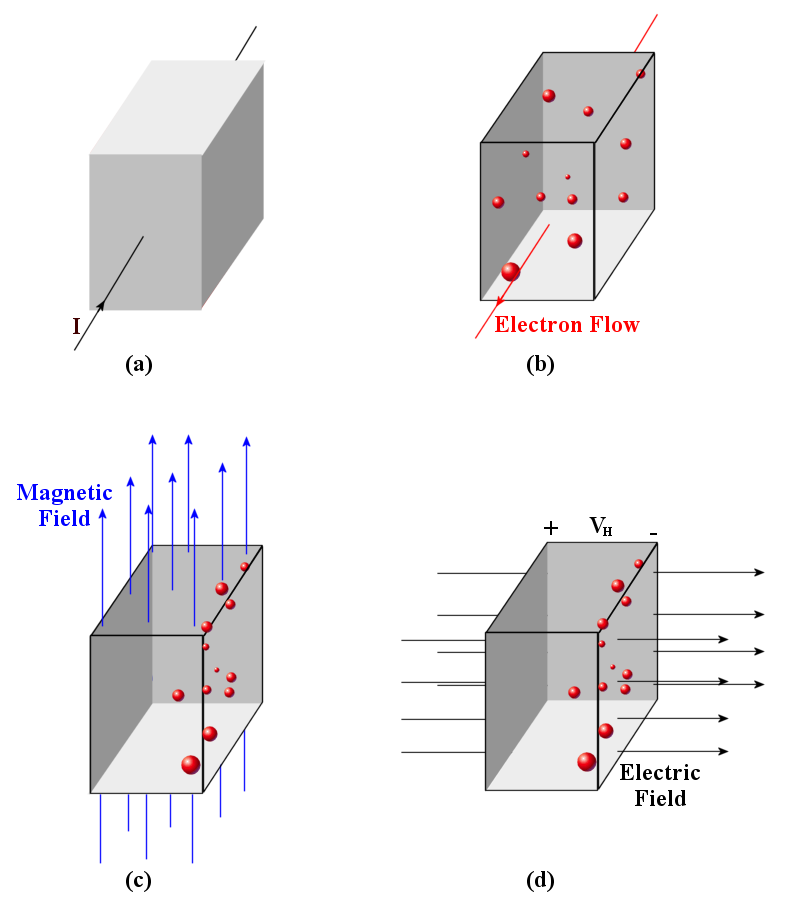
\includegraphics[width=\linewidth,height=\linewidth]{shift-electrons.png}
\caption{a). Representation of the general setup wiyh the sample and a wire 
providing current through the sample. b). A general representation of the flow 
of electrons in the sample. c). The general shift in the position of the 
electrons as they pass through a magnetic field. d). Electric field that is 
produced when the electrons distribute themselves in such a manner 
\cite{ref:2}.}
\label{fig:1}
\end{minipage}
\hfill
\begin{minipage}[t]{0.46\textwidth}
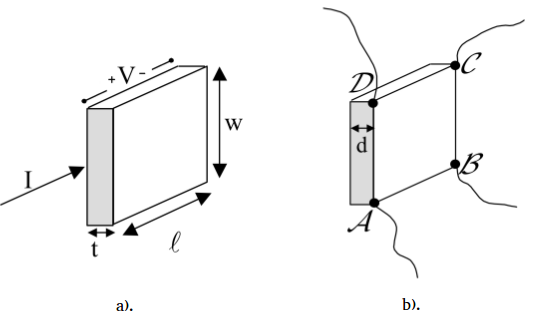
\includegraphics[width=\linewidth]{contacts-dim.png}
\caption{a). Current passing through a sample of dimension l,w,t. b). Sample of
depth d with four contacts placed on the corners of the sample.}
%\cite{ref:3}
\label{fig:2}
\end{minipage}
\end{figure*}
%\end{wrapfigure}
From electricity and magnetism we know that charged particles passing through 
a magnetic field display the following force relation,
\begin{equation}
\label{eqn:1}
\vec{F}=q(\vec{E}+\vec{v}\times\vec{B})
\end{equation}
Where, q is the charge of the particle, $\vec{E}$ is the electric field 
in the space of the particle, $\vec{v}$ is its velocity and $\vec{B}$ is the 
magnetic field. Usually, we can consider the contribution of the electric field 
to the force to be zero so we can write equation \ref{eqn:1} as,
\begin{equation}
\label{eqn:2}
\vec{F}=q\vec{v}\times\vec{B}
\end{equation}
So that is to say that the charge carriers will receive a force that is 
perpendicular to their motion and as a cause will begin to curve. If we now 
think about a solid material through which we pass some current it would look 
like figure \ref{fig:1}b. Where the electrons are free to move through the 
entire sample and have nothing directing their movement other than the electric 
current that is passing through the sample. For a pictorial representation of 
what happend when we apply a strong magnetic field perpendicular to the sample 
refer to figures \ref{fig:1}c,d. This makes sense with equation \ref{eqn:2} and 
what we generally know of charged particles passing through a perpendicular 
magnetic field. Looking at figure \ref{fig:1}d the reason why it does in fact 
produce an electric field inside of the sample is due to the electrons that 
have curved to a side of the sample and since they can't conduct very easily 
through the a air they accumulate at the boundary of the sample toward which 
they curve creating a gradient of electrons and lack of electrons (positive 
charge) which gives rise to a potential difference through the sample and 
therefore an electric field through the sample.
\\
This perpendicular magnetic field can be calculated with equation \ref{eqn:3}.
\begin{equation}
\vec{E}_t = \frac{-\vec{J}\times\vec{B}}{nq}
\cite{ref:1}
\label{eqn:3}
\end{equation}
Where, $\vec{J}$ is the current density, $\vec{B}$ is the magnetic field 
passing through the sample,n is the number carriers and q is the charge of the 
carriers.
\\
Equation \ref{eqn:3} is mainly useful were qe to know all of the 
parameters we need which, for this experiment, we need to find. So we take a 
different approach in our equation derivations starting with how to calculate 
the resistivity of a semiconductor sample.
\\
When we have a sample with a current passing through it of certain current 
density, j, We can show that the electric field is related in the following way,
\begin{equation}
\vec{E} = \rho\vec{j}
\cite{ref:3}
\label{eqn:4}
\end{equation}
Where, $\rho$ is the resistivity of the sample. By multiplying both sides of 
equation \ref{eqn:3} by the length of the sample, l, we can get a relation 
between the voltage and the resistivity.
\begin{equation}
V = \rho\frac{l}{tw} I 
\cite{ref:3}
\label{eqn:5}
\end{equation}
Where, l,t,w are the dimensions shown of figure \ref{fig:2}b and I is the 
total current through the sample. By then applying Ohm's law, V=IR, we can get 
to the relation of resistance with resistivity.
\begin{equation}
R = \rho\frac{l}{wt} = R_s\frac{l}{w}
\cite{ref:3}
\label{eqn:6}
\end{equation}
Where, $R_s = \rho/t$. $R_s$ is the sheet resistance of the sample and it is 
only dependent on the thickness of the sample as per the equation. Notice that 
if the sample is perfectly square, l=w, $R_s = R$ \cite{ref:3}. By performing a 
two contact resistivity measurement we can receive values for the resistivity 
of the sample. However, as it will be more apparent later these values that we 
get do have a certain amount of error and a more accurate method can be 
employed. This method is the va der Pauw method which was developed in 1958 by 
Leo J. van der Pauw.
\\
To use this method the following conditions must be met \cite{ref:4}.
\begin{enumerate}[label=\alph*]
\item The contacts are at the circumference of the sample.
\item The contacts are sufficiently small.
\item The sample is homogeneous in thickness.
\item The surface of the sample is singly connected,i.e.,the sample does not 
have isolated holes.
\end{enumerate}
Now, the first condition assumes that the sample is a disc, but this method can 
work for any shape like a square. The derivation of the method can be found in 
\cite{ref:3}
Now, the first condition assumes that the sample is a disc, but this method can 
work for any shape like a square. The derivation of the method can be found in 
\cite{ref:3}. In figure \ref{fig:2}b we see that the contacts are placed in the 
corners. They do not have to necessarily be on the corners. They can be 
anywhere along the edge of the sample. According to van der Pauw's paper the 
resistivity of a sample using the four contact method can be calculated with 
the following equation.
\begin{equation}
\rho = \frac{\pi d}{\ln{2}}\frac{R_{AB,CD}+R_{BC,DA}}{2}f\left(\frac{R_{AB,CD}}{R_{BC,DA}}\right)
\cite{ref:4}
\label{eqn:7}
\end{equation}
\begin{figure*}
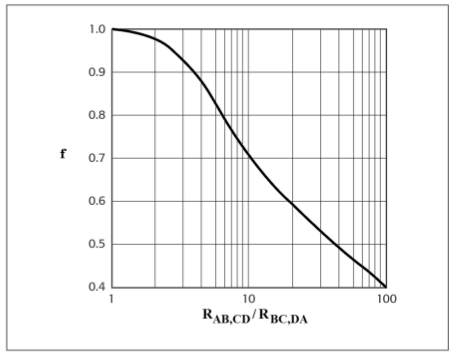
\includegraphics[width=\textwidth,height=3.5in]{f-function.png}
\caption{Plot of the f function from equation \ref{eqn:6} \cite{ref:3}.}
\label{fig:3}
\end{figure*}
Where, d is the thickness of the sample (t in the case of fig. \ref{fig:2}b), 
$R_{AB,CD}$ and $R_{BC,AD}$ represent current passing through the point and 
making the voltage measurement respectively. That is to say they are along the 
perpendicular current directions as can be inferred from figure \ref{fig:2}b. 
The function f is a function that behaves in 
similar fashion to that which is shown on figure \ref{fig:3}. Where it only 
satisfies the relation.
\begin{equation}
\frac{R_{AB,CD}-R_{BC,DA}}{R_{AB,CD}+R_{BC,DA}} = f\arccosh{\frac{\exp{\ln{2/f}}}{2}}
\cite{ref:4}
\label{eqn:8}
\end{equation}
Which can only be solved numerically to solve for f. Van der Pauw does provide 
another equation to approximate f where the ratio of $R_{AB,CD}/R_{BC,DA}$ are 
almost equal.
\begin{equation}
\begin{split}
f \approx 1-\left(\frac{R_{AB,CD}-R_{BC,DA}}{R_{AB,CD}+R_{BC,DA}}\right)^2\frac{\ln{2}}{2}- \\
\left(\frac{R_{AB,CD}-R_{BC,DA}}{R_{AB,CD}+R_{BC,DA}}\right)^4\left\{\frac{(ln{2})^2}{4}-\frac{(\ln{2})^2}{12}\right\}
\cite{ref:4}
\label{eqn:9}
\end{split}
\end{equation}
There is another method that can be used in which we use a table which is 
provided to us. However, to reduce errors from approximating to the second 
decimal point the f value is calculated for every ratio and was compared to the 
given f values. They agreed to the second decimal and was believed to be a 
better approximation than those given in the table.
\\
In general, we can represent the resistivity and conductivity of a sample of 
comparable size as a tensor meaning that the electric field and the current 
density may not necessarily be parallel to one another. Such matrices are the 
following.
\begin{equation*}
\begin{align*}
\rho &= 
\begin{bmatrix}
\rho_{xx}&\rho_{xy} \\
-\rho_{xy}&\rho_{yy}
\end{bmatrix}
\\
\sigma &= 
\begin{bmatrix}
\sigma_{xx}&\sigma_{xy} \\
-\sigma_{xy}&\sigma_{yy}
\end{bmatrix}
\end{align*}
\end{equation*}
Where, the x and y subscripts represent the sheet coordinate directions of the 
sample ignoring the z.
\\
Back in equation \ref{eqn:3} we showed the relation between the current density 
and the magnetic field to find the electric field that is produced by the Hall 
Effect. Here, a different form of it will be shown using vectors and tensors.
\begin{equation}
\begin{bmatrix}
E_{x}\\E_{y}
\end{bmatrix}
=
\begin{bmatrix}
\rho_{xx}&\rho_{xy} \\ 
-\rho_{xy}&\rho_{yy}
\end{bmatrix}
\begin{bmatrix}
j_x \\ 0
\end{bmatrix}
\cite{ref:3}
\label{eqn:10}
\end{equation}
Where, $j_y = 0$ since there is no input current along the y direction of the 
sample only along the x direction. When equation \ref{eqn:10} is solved for the 
electric field components we can get the following equations.
\begin{equation}
\begin{align*}
E_x &= \rho_{xx}j_x\\
E_y &= -\rho_{xy}j_x
\cite{ref:3}
\label{eqn:11}
\end{align*}
\end{equation}
Where, if we transform equation \ref{eqn:11} as we did with equation 
\ref{eqn:4} we get a 
relation between $V_Hall$ and the xy resistance of the sample. Keep in mind 
that it is the Hall voltage as the field in the y direction is a direct cause 
of the magnetic filed that is along the z direction.
\begin{equation}
V_{Hall} = R_{xy}I
\cite{ref:3}
\label{eqn:12}
\end{equation}
Where, $R_{xy}$ is given by the equation.
\begin{equation}
R_{xy} = \frac{R_H}{t}B
\cite{ref:3}
\label{eqn:12}
\end{equation}

\begin{thebibliography}{9}
\bibitem{ref:1}
Purcell, E. M.; Morin, D. J. (2013). Electricity and Magnetism. New York: 
\emph{Cambridge University Press}, 314-317.
\bibitem{ref:2}
(2016,December 24).Van der Pauw method. \emph{Wikipedia}. 
https://en.wikipedia.org/wiki/\\Van\_der\_Pauw\_method
\bibitem{ref:3}
UB 2015 Lab Manual. Hall Effect
\bibitem{ref:4}
van der Pauw, L. J. (1958). A method of measuring specific resistivity and 
Hall Effect of discs of arbitrary shape. \emph{Philips Research reports, 13}, 
1-9.
\end{thebibliography}
\end{document}
